\begin{center}
\large \textbf{Písemná práce:} exponenciální funkce \textbf{(varianta A)}

\normalsize
\makebox[8cm]{\textsc{Jméno:}\enspace\hrulefill}\qquad
\makebox[3cm]{\textsc{Třída:}\enspace\hrulefill}\qquad
\makebox[4cm]{\textsc{Datum:}\enspace\hrulefill}
\end{center}
\begin{table}[h]
\centering
\begin{tabular}{c|c|c|c|c|c}
    \textbf{Body}   & $< 9$ & $8-7$ & $6-5$ & $4-3$ & $2-0$ \\ \hline
    \textbf{Známka} & $1$     & $2$   & $3 $  & $4$   & $5$
\end{tabular}
\end{table}

\noindent
% First Question
\begin{questions}
    \bracketedpoints

    \question[1] Napište definici exponenciální funkce.
                \fillwithdottedlines{3\dottedlinefillheight}
    \question[1] Stručně vysvětlete, proč klademe na hodnotu základu exponenciální funkce omezení.
                \fillwithdottedlines{3\dottedlinefillheight}
    \question[2] Vyberte funkční předpis odpovídající grafu funkce $f$ níže.\\
    \begin{center}
        \begin{tikzpicture}[>=latex]
            \begin{axis}[
            x=1cm,y=1cm,
            axis x line=center,
            axis y line=center,
            xtick={-3,-2,...,5},
            ytick={-2,-1,...,3},
            minor tick num=1,
            xlabel={$x$},
            ylabel={$y$},
            xlabel style={below right},
            ylabel style={above left},
            xmin=-2.9,
            xmax=3.4,
            ymin=-1.4,
            ymax=3.4,
            anchor=center]
                \addplot [domain=-2.8:3.3] {(1/2)^(x+1)-1} node[pos=1] (endofplotsquare) {};
                \node [above,color=black] at (endofplotsquare) {$f$};
                \node[label={180:{$-\frac{1}{2}$}},inner sep=2pt] at (axis cs:0,-0.5) {};
                \addplot [dotted,mark=none] {-1};
                \addplot [dotted,mark=none,domain=-2:0] {1};
                \addplot [dotted,mark=none,domain=0:1] coordinates {(-2,0)(-2,1)};
                \node[circle,fill,inner sep=2pt,scale=0.5] at (axis cs:-2,1) {};
            \end{axis}
        \end{tikzpicture}
    \end{center}

    \begin{checkboxes}
        \choice $f: y=\left(\tfrac{1}{2}\right)^{x-1}+1$
        \CorrectChoice $f: y=\left(\tfrac{1}{2}\right)^{x+1}-1$
        \choice $f: y=2^{x-1}+1$
        \choice $f: y=2^{x+1}-1$
        \choice Žádný z uvedených.
    \end{checkboxes}

    \newpage

    \question[6] Mějme reálnou funkci $g: y=-2^{x-2}+\tfrac{1}{2}$, kde $D_g=\left(-4,3\right\rangle$. %Ke  každé části uveďte postup řešení.
    \begin{parts}
        \renewcommand{\thepartno}{\Alph{partno}}
        \part[4] Nakreslete graf funkce $g$.
        \part[1] Určete obor hodnot $H_g$.
        \part[1] Určete průsečík grafu $g$ s osou $x$ a $y$.
    \end{parts}
    \begin{center}
        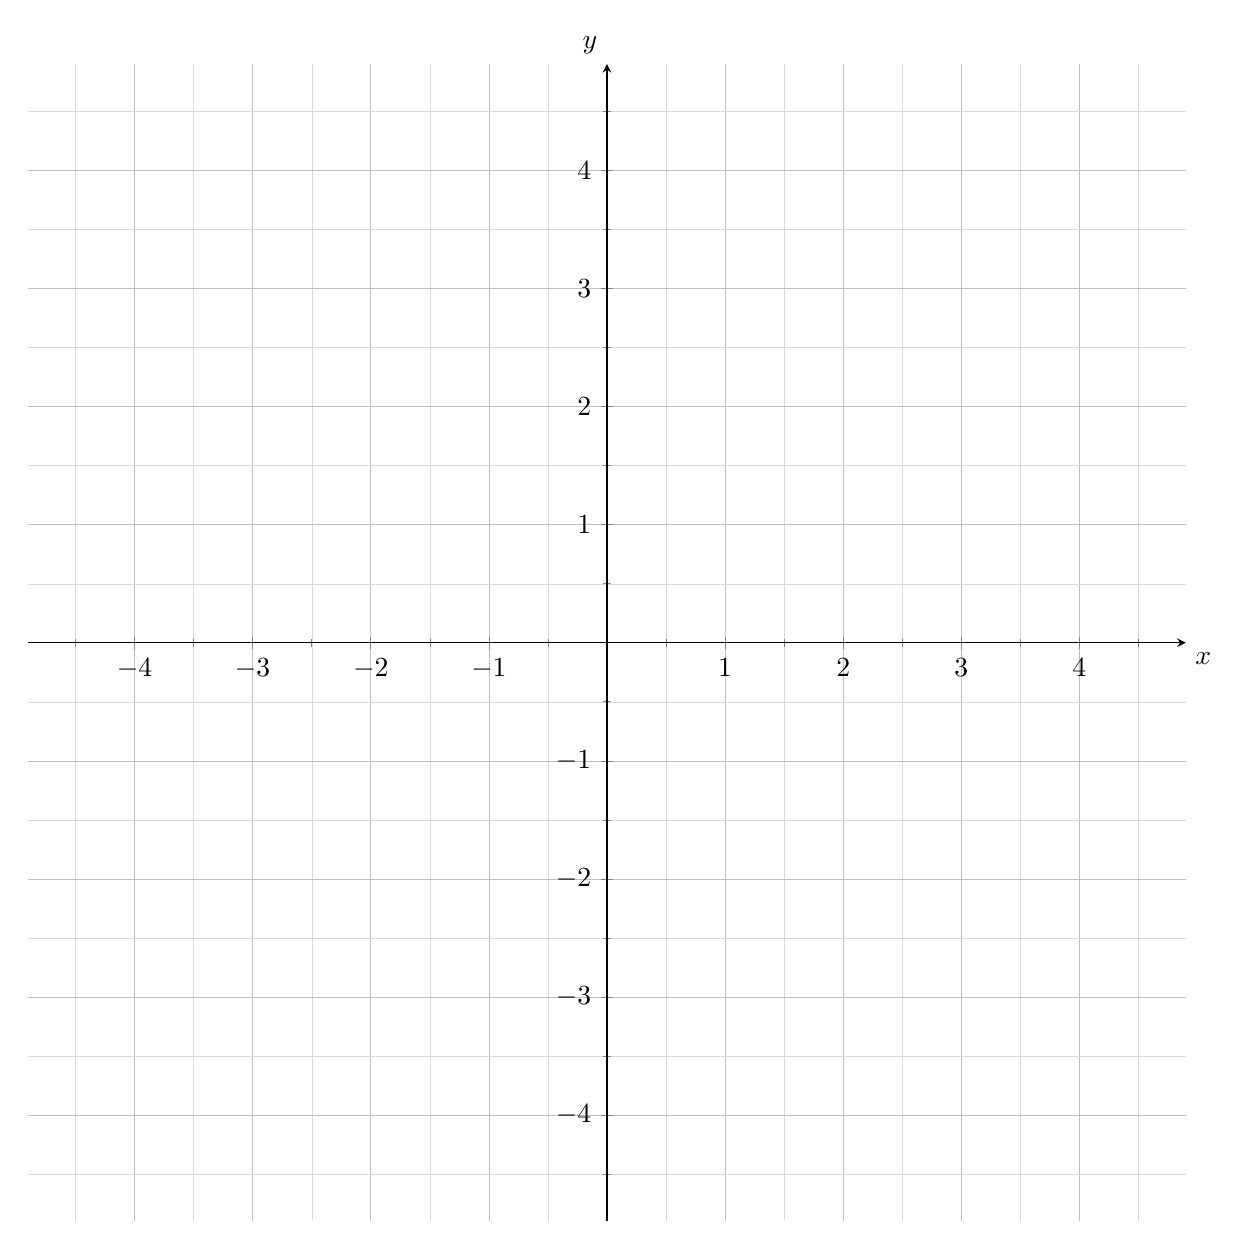
\begin{tikzpicture}[>=latex]
            \begin{axis}[
            x=1.5cm,y=1.5cm,
            axis x line=center,
            axis y line=center,
            xtick={-5,-4,...,5},
            ytick={-5,-4,...,5},
            minor tick num=1,
            grid=both,
            grid style={line width=.1pt, draw=gray!30},
            major grid style={line width=.2pt,draw=gray!50},
            xlabel={$x$},
            ylabel={$y$},
            xlabel style={below right},
            ylabel style={above left},
            xmin=-4.9,
            xmax=4.9,
            ymin=-4.9,
            ymax=4.9,
            anchor=center]
            \end{axis}
        \end{tikzpicture}
    \end{center}
    \newpage

    \bonusquestion[4] Mějme reálnou funkci $h: y=\left(\tfrac{a+1}{a^2-1}\right)^x$. Určete, pro jaké hodnoty parametru $a\in\R$ je funkce $h$ klesající. Uveďte celý postup řešení.
    \newpage
\end{questions}

\begin{center}
\Large\textbf{Vzorové řešení}\normalsize
\begin{enumerate}
    \item Nechť $a \in \mathbb{R}^+ \setminus \{ 1 \}$. Exponenciální funkcí i základu $a$ se nazývá funkce $f$ daná rovnicí $y=a^x$, jejím definičním oborem je $D(f) = \mathbb{R}$.

    \item Pro $a=1$ je $y=1^x = 1$ pro každé $x \in \mathbb{R}$, tj. funkce je konstantní, proto tento případ u exponenciální funkce vylučujeme.
    Pokud by základ byl záporný, např. mějme funkci $f(x) = (-2)^x$. Když za $x$ dosadíme $\tfrac{1}{2}$, dostaneme $y=(-2)^{\tfrac{1}{2}} = \sqrt{-2}$. My ale víme, že odmocnina ze záporného čísla v $\mathbb{R}$ neexistuje. Funkce by tak nebyla definovaná na celém $\mathbb{R}$.

    \item $f: y=\left(\tfrac{1}{2}\right)^{x+1}-1$
    \item Graf:\\
    \begin{center}
        \begin{tikzpicture}[>=latex]
            \begin{axis}[
            x=1cm,y=1cm,
            axis x line=center,
            axis y line=center,
            xtick={-4,-3,...,3},
            ytick={-2,-1,...,3},
            minor tick num=1,
            xlabel={$x$},
            ylabel={$y$},
            xlabel style={below right},
            ylabel style={above left},
            xmin=-4.3,
            xmax=3.7,
            ymin=-2.4,
            ymax=1.4,
            anchor=center]
                \addplot [domain=-4:3] {-2^(x-2)+(1/2)} node[pos=1] (endofplotsquare) {};
                \node [above,color=black] at (endofplotsquare) {$g$};
                \addplot [dotted,mark=none] {0.5};
                \coordinate (begin) at (axis cs:-4,31/64);
                \coordinate (end) at (axis cs:3,-3/2);
            \end{axis}
            \filldraw[draw=black,fill=white]  (begin) circle(0.7mm);
            \filldraw[fill=black,draw=black] (end) circle(0.7mm);

        \end{tikzpicture}
    \end{center}

    $$H_g = \left(-\tfrac{31}{64},\tfrac{-3}{2}\right\rangle$$
    $$P_x = \left[1,0\right]$$
    $$P_y = \left[0,\tfrac{1}{4}\right]$$
    \item Funkce $h$ má být klesající, tj. $0<\frac{a+1}{a^2-1}<1$. Každou z nerovností vyšetříme zvlášť:
    \begin{align*}
    0&<\frac{a+1}{a^2-1}\\
    0&<\frac{1}{a-1}\; ; \; a\neq -1\\
    a&\in(1,\infty).
    \end{align*}
    Druhá nerovnost:
    \begin{align*}
    \frac{a+1}{a^2-1}&<1\\
    0&<1-\frac{a+1}{a^2-1}\\
    0&<\frac{a^2-a-2}{a^2-1}\\
    0&<\frac{(a-2)\cancel{(a+1)}}{(a-1)\cancel{(a+1)}}\\
    \end{align*}
    \begin{table}[H]
    \centering
    \begin{tabular}{c|c|c|c}
            & $(-\infty,1)$ & $(1,2)$ & $(2,\infty)$ \\ \hline
    $a-1$ & -             & +       & +            \\ \hline
    $a-2$ & -             & -       & +            \\ \hline
            & +             & -       & +
    \end{tabular}
    \end{table}
    Tj. $a\in\R\setminus\big((1,2)\cup\set{-1}\big)$.
    Parametr $a$ tedy náleží průniku $\Big(\R\setminus\big((1,2)\cup\set{-1}\big)\Big)\cap(1,\infty)=(2,\infty)$.
\end{enumerate}
\end{center}
